\documentclass[aspectratio=1610,xcolor=dvipsnames]{beamer}
\usepackage{theme}
\usepackage[utf8x]{inputenc}

\usepackage[english]{babel}
\usepackage{calligra}
\usepackage{subcaption}
\usepackage{hyperref}

\usepackage{amsmath,amssymb,amsfonts}
\usepackage{array, booktabs, makecell}
\usepackage{tabularx}

\usepackage{textcomp}
\usepackage[ruled]{algorithm2e}
\makeatletter
\newcommand{\removelatexerror}{\let\@latex@error\@gobble}
\makeatother

% Graphics and video
\usepackage{graphicx,float,wrapfig}
\usepackage{animate}
\graphicspath{
  {../assets/}%
}

% args: big, bigg, Big, Bigg
\newcommand{\parenth}[2][]{#1(#2#1)}
\renewcommand{\bold}[1]{\textbf{\structure{#1}}}
  
\author[Conti \and Daniotti]{Samuele Conti \and Filippo Daniotti}
\title[Global Motion Estimation]{\textsc{Global Motion Estimation}}
\subtitle{An indirect, multiscale and robust approach}
\institute[DISI - UniTN]{Department of Information Engineering\\and Computer Science}
\date{April 20, 2022}


\AtBeginSection[]
{
    \begin{frame}
        \frametitle{Table of Contents}
        \tableofcontents[currentsection]
    \end{frame}
}

\begin{document}

\begin{frame}
    \titlepage
    \begin{figure}[H]
        \begin{center}
            
\includegraphics[width=0.4\linewidth]{marchio_unitrento_colore_it_202002.eps}
        \end{center}
    \end{figure}
\end{frame}

\begin{frame}
    \tableofcontents[sectionstyle=show,subsectionstyle=show/shaded/hide,subsubsectionstyle=show/shaded/hide]
\end{frame}

\section{Introduction}
\begin{frame}{Introduction}
    In this work we are going to present:
    \begin{itemize}
        \item a broad introduction to the problem of global motion estimation
        \item an overview of the theoretical foundations of our solution
        \item the framework we developed from the aforementioed literature
        \item an analysis of the results of our solution 
    \end{itemize}
\end{frame}

\section{The problem}
\begin{frame}{Global motion estimation}
    The motion in videos can be analyzed as the displacement of pixel per pair of frames
    \bigskip

    \begin{columns}
        \begin{column}{0.45\textwidth}
            Is usually the combination of two different motions:
            \begin{itemize}
                \item the actual motion of objects in the scene
                \item the egomotion of the camera
            \end{itemize}
        \end{column}
        \begin{column}{0.45\textwidth}
            \begin{figure}[H]
                \animategraphics[loop,autoplay,width=.6\linewidth]{20}{gifs/pan240/pan240-}{0}{40}
                \caption{Local motion vs. egomotion}
            \end{figure}
        \end{column}
    \end{columns}

    \begin{alertblock}{The problem}
        Global motion estimation aims to extract the camera global motion patterns in a video
    \end{alertblock}
\end{frame}

\begin{frame}{Motion models}
    Motion models describe camera motion patterns through equations
    \bigskip
    \begin{columns}
        \begin{column}{0.35\textwidth}
            \begin{figure}
                \centering
                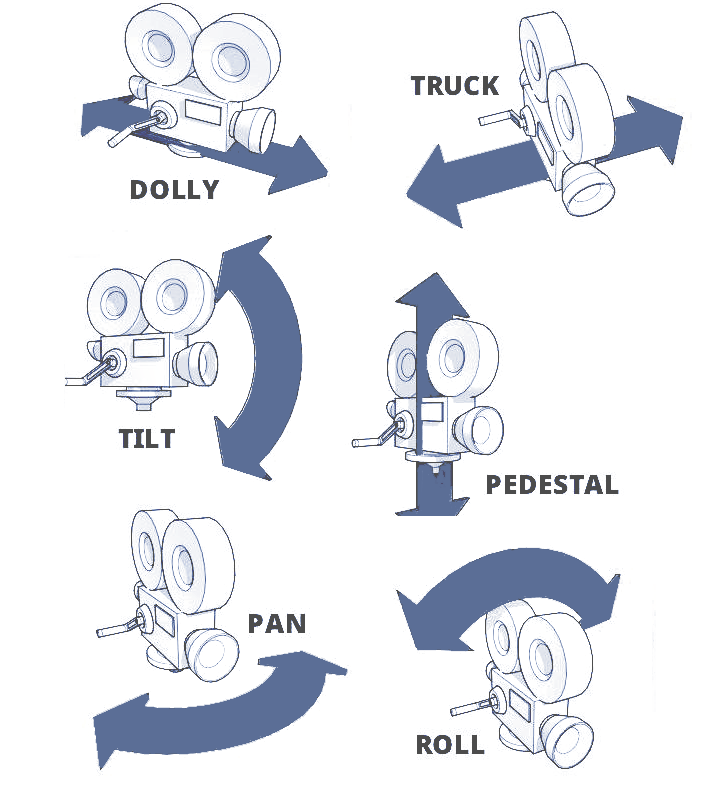
\includegraphics[width=.9\linewidth]{../assets/images/camera-movement.png}
                \caption{Different models describe different types of camera motion}
                \label{fig:camera-motion}
            \end{figure}
        \end{column}
        \begin{column}{0.65\textwidth}
            The displacement of a pixel across frames as a function of some parameters
            \begin{equation}
    \label{eq:affine-model-representation}
    p' = 
    \begin{bmatrix}
        X' \\ Y' \\ Z'
    \end{bmatrix}
    =
    \begin{bmatrix}
        r_1 & r_2 & r_3 \\
        r_4 & r_5 & r_6 \\
        r_7 & r_8 & r_9 
    \end{bmatrix}
    \begin{bmatrix}
        X \\ Y \\ Z
    \end{bmatrix}
    +
    \begin{bmatrix}
        T_X \\ T_Y \\ T_Z
    \end{bmatrix}
    = Rp + T
\end{equation}
            E.g. the \bold{affine model} (our choice) has the following simplified form 
            \begin{equation}
    \label{eq:affine-model-representation}
    \begin{bmatrix}
        d_x(x,y) \\ d_y(x,y)
    \end{bmatrix}
    =
    \begin{bmatrix}
        a_0 + a_1 x + a_2 y \\
        b_0 + b_1 x + b_2 y
    \end{bmatrix}
\end{equation}
        \end{column}
    \end{columns}
\end{frame}

\begin{frame}{Estimating parameters}
    There are two main approaches, both of which aim to minimize a prediction error
    \bigskip
    \begin{itemize}
        \item \bold{direct methods} work in the pixel domain
        \item \bold{indirect methods} work with motion fields
    \end{itemize}
    \bigskip
    For our solution we opted for \bold{indirect methods}
    \begin{block}{Indirect parameter update}
        The parameter vector \(a\) is updated by choosing the parameters that minimize the dissimilarity of the \(gt(p)\) and the prediction \(MM(p,a)\) for a point \(p\)
        \begin{equation}
    \label{eq:indirect-estimation}
    a = \arg \min_a \sum_p E(gt(p) - MM(p, a))
\end{equation}
    \end{block}
\end{frame}

\section{Implementation}
\begin{frame}{Overview}
    \begin{columns}
        \begin{column}{0.45\textwidth}
            \begin{figure}[H]
                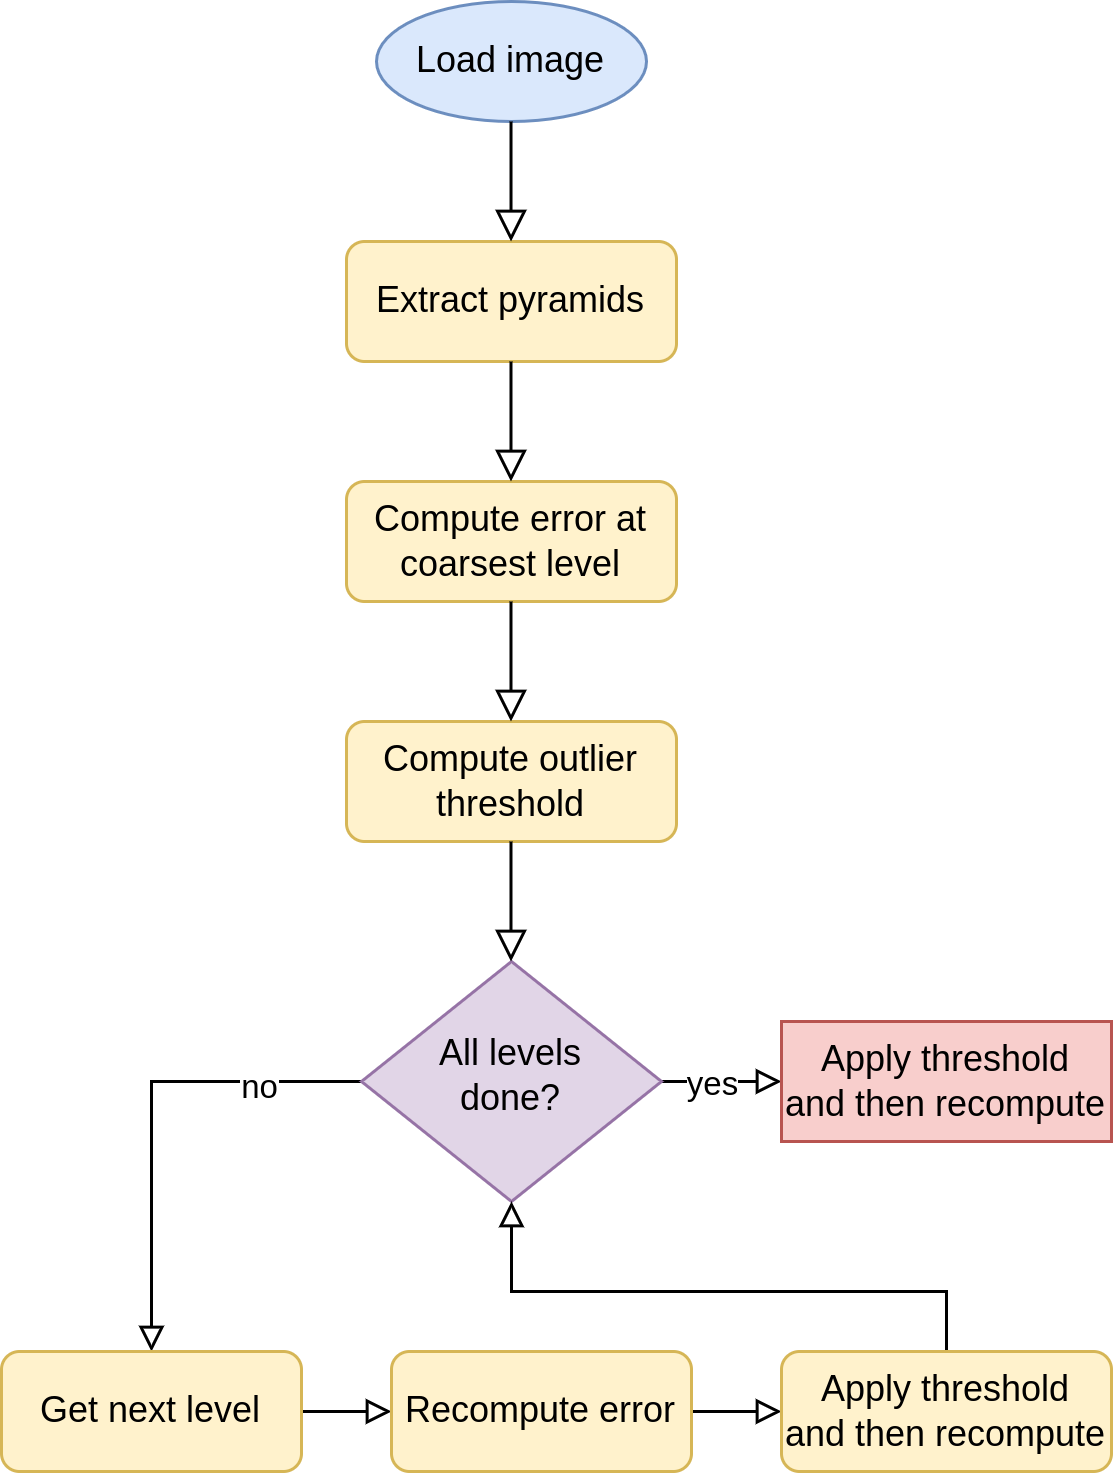
\includegraphics[keepaspectratio,width=.8\textwidth]{images/implementation-flow.png}
                \caption{Flowchart of our framework}
            \end{figure}
        \end{column}
        \begin{column}{0.45\textwidth}
            Implementation choices:
            \begin{itemize}
                \item Affine model
                \item Indirect method
                \item Block-based motion estimation
                \item Multiscale
                \item Robust
            \end{itemize}
        \end{column}
    \end{columns}
\end{frame}

\subsection{Block-based motion estimation}
\begin{frame}{Block-based motion estimation}
	BBME algorithms perform motion estimation and return the motion field to use as ground truth for indirect parameter estimation

	\bigskip	
    \begin{exampleblock}{Chosen algorithms}
        We implemented 4 well-known BBME algorithms:
        \begin{itemize}
            \item exhaustive search
            \item three-step search
            \item 2D log search
            \item diamond search
        \end{itemize}        
    \end{exampleblock}
\end{frame}

\begin{frame}{Exhaustive search}
	\begin{figure}
		\begin{minipage}{.45\textwidth}
            \centering
            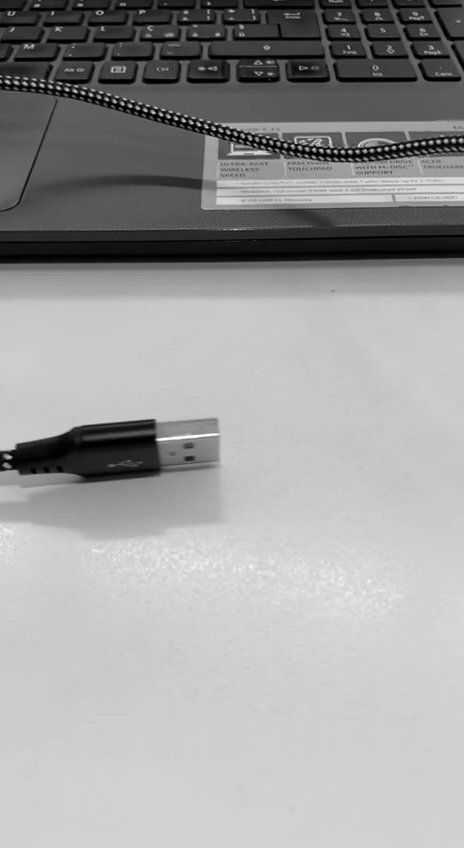
\includegraphics[keepaspectratio, width=.55\linewidth]{images/bbme-im.png}
            \subcaption{Target frame}
            \label{fig:bbme-0-im}
		\end{minipage}
		\begin{minipage}{.45\textwidth}
            \centering
            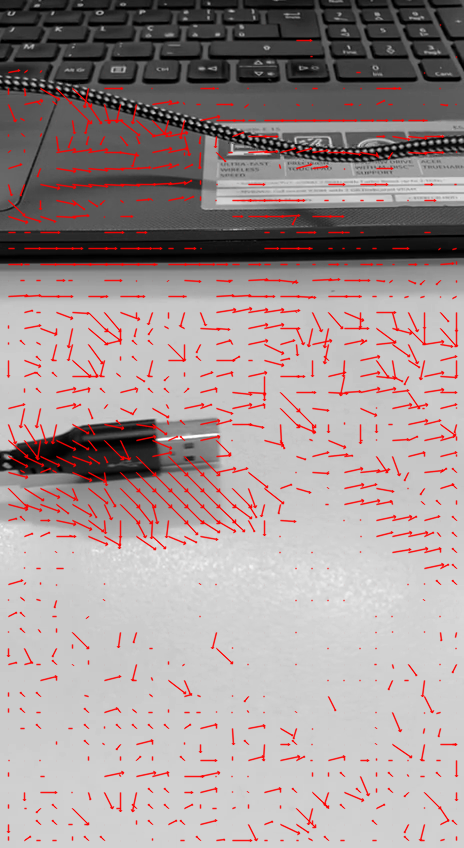
\includegraphics[keepaspectratio, width=.55\linewidth]{images/bbme-0-res.png}
            \subcaption{Needle diagram}
            \label{fig:bbme-0-res}
		\end{minipage}
        \label{fig:bbme-0}
        \caption{Motion field result of our EBBME implementation}
	\end{figure}
\end{frame}

\begin{frame}{Three-step search}
	\begin{figure}[H]
		\begin{minipage}{.45\textwidth}
            \centering
            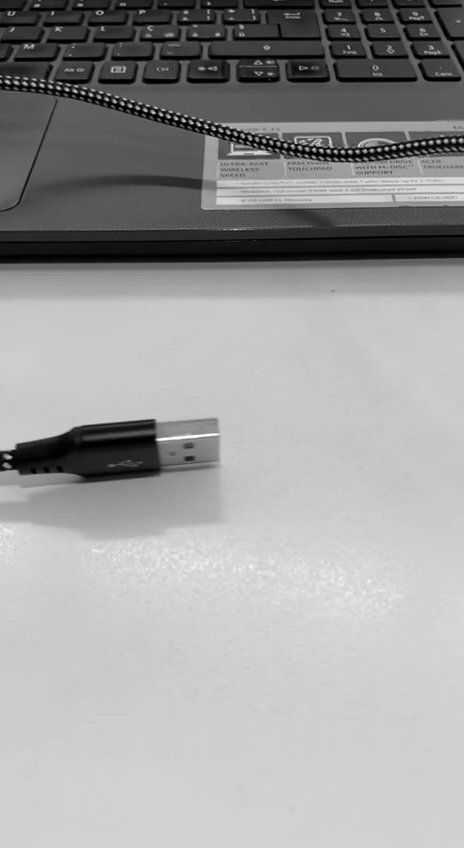
\includegraphics[keepaspectratio, width=.55\linewidth]{images/bbme-im.png}
            \subcaption{Target frame}
            \label{fig:bbme-1-im}
		\end{minipage}
		\begin{minipage}{.45\textwidth}
            \centering
            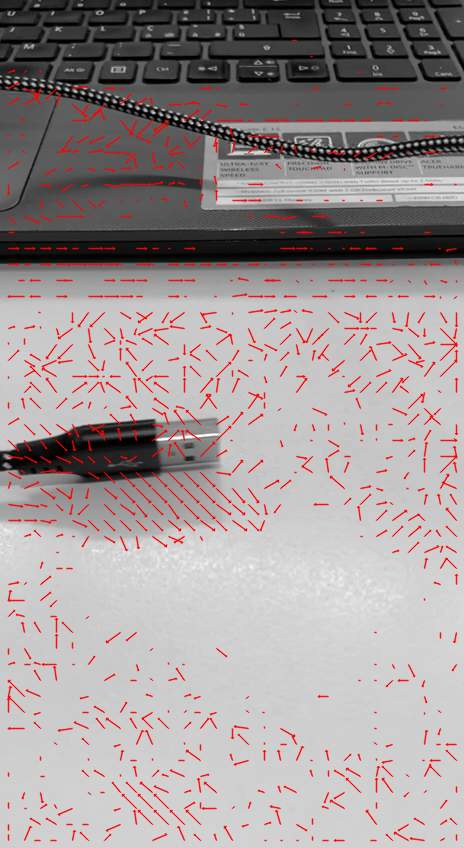
\includegraphics[keepaspectratio, width=.55\linewidth]{images/bbme-1-res.png}
            \subcaption{Needle diagram}
            \label{fig:bbme-1-res}
		\end{minipage}
		% \begin{minipage}{.3\textwidth}
        %     \centering
        %     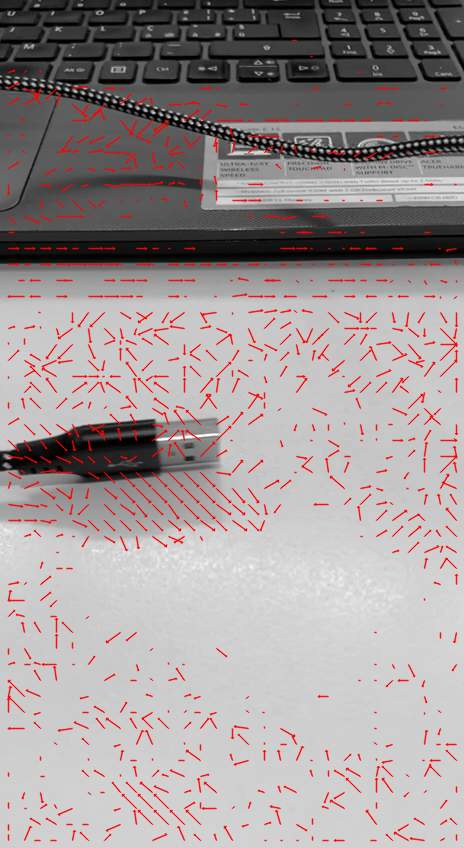
\includegraphics[keepaspectratio, width=.8\linewidth]{images/bbme-1-res.png}
        %     \subcaption{Hierarchical version}
        %     \label{fig:bbme-h1-res}
		% \end{minipage}
        \label{fig:bbme-1}
        \caption{Motion field result of our TSS implementation}
	\end{figure}
\end{frame}

\begin{frame}{2D Log search}
	\begin{figure}
		\begin{minipage}{.45\textwidth}
            \centering
            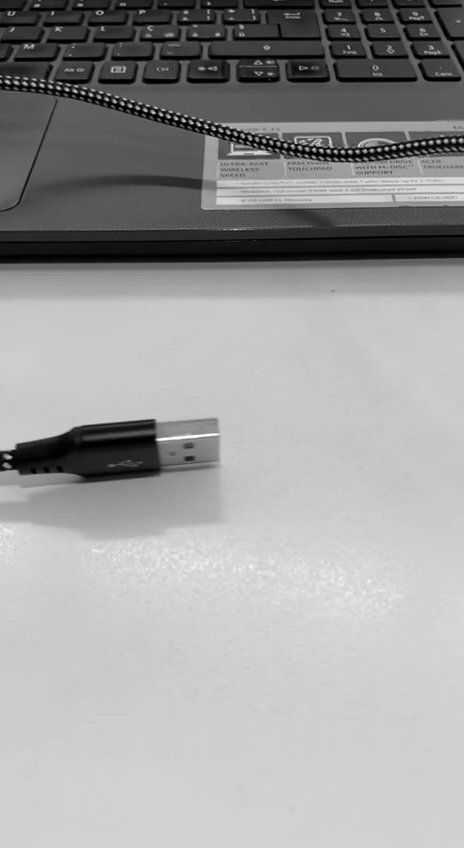
\includegraphics[keepaspectratio, width=.55\linewidth]{images/bbme-im.png}
            \subcaption{Target frame}
            \label{fig:bbme-2-im}
		\end{minipage}
		\begin{minipage}{.45\textwidth}
            \centering
            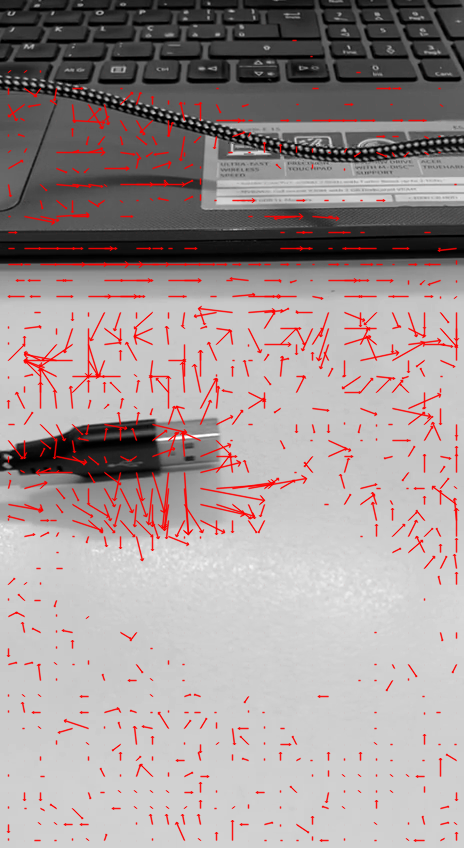
\includegraphics[keepaspectratio, width=.55\linewidth]{images/bbme-2-res.png}
            \subcaption{Needle diagram}
            \label{fig:bbme-2-res}
		\end{minipage}
        \label{fig:bbme-2}
        \caption{Motion field result of our TDLS implementation}
	\end{figure}
\end{frame}

\subsubsection*{Diamond search BBME}
\begin{frame}{Diamond search}
	BBME algorithm presented in Zhu and Ma, 2000. 
    \bigskip
    
    Better performances thant classic algorithms (TSS) and comparable to latest ones (NTSS), yet more efficient in computation.
    \bigskip
    \begin{columns}
        \begin{column}{0.5\textwidth}
            It uses two different  diamond-shaped search patterns:
            \begin{itemize}
                \item large diamond search pattern (LDSP)
                \item small diamond search pattern (SDSP)
            \end{itemize}
        \end{column}
        \begin{column}{0.5\textwidth}
            \begin{figure}
                \centering
                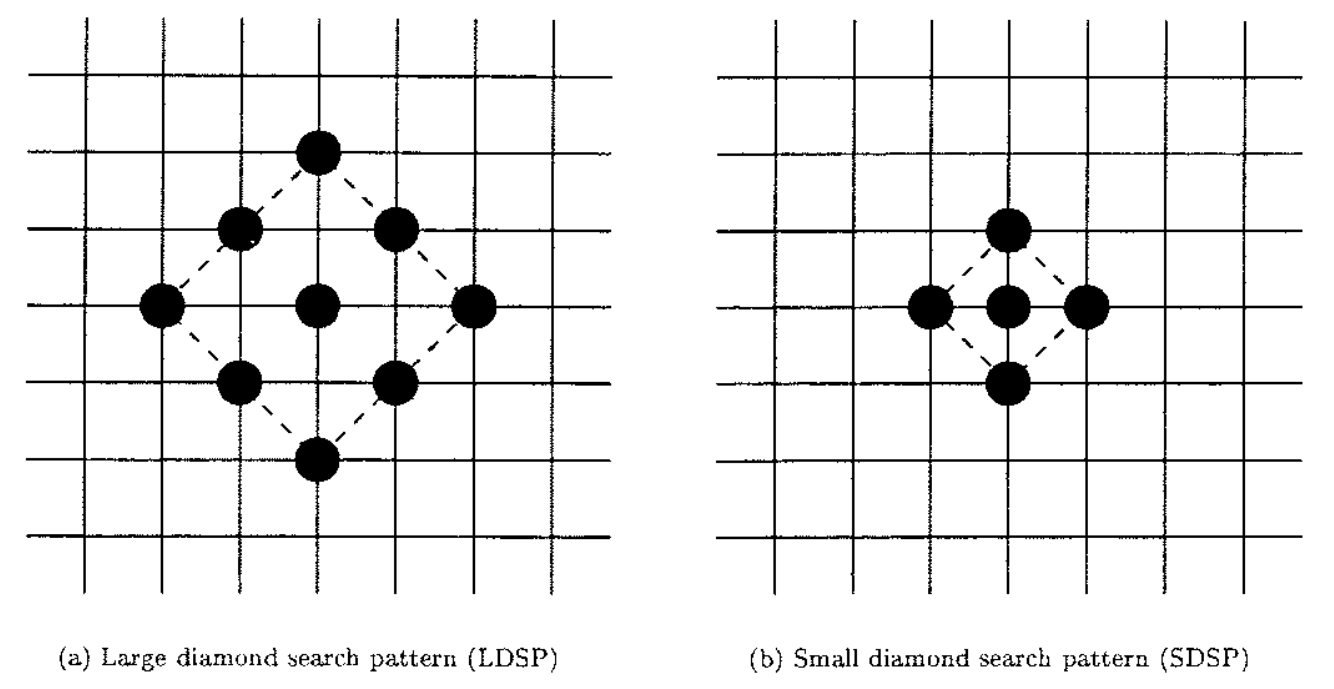
\includegraphics[keepaspectratio,width=\linewidth]{images/ds-search-patterns.png}
                \caption{The shape of LDSP and SDSP}
            \end{figure}
        \end{column}
    \end{columns}
\end{frame}

\begin{frame}{DS algorithm}
    \begin{block}{Diamond search procedure}
        For each block:
        \begin{enumerate}
            \item place LDSP in the center of the block and compute DFD for all of the 9 displacements;
            \begin{itemize}
                \item if the minimum DFD is in the center position, then go to 3
                \item else, go to 2
            \end{itemize}
            \item reposition LDSP in the minimum DFD of the previous operation and recompute DFD;
            \begin{itemize}
                \item if the minimum DFD is in the center position, then go to 3
                \item else, repeat 
            \end{itemize}
            \item place SDSP, compute DFD and return coordinates of the minum DFD block as motion vector
        \end{enumerate}
    \end{block}
\end{frame}

\begin{frame}{DS algorithm visualized}
    \begin{figure}
        \centering
        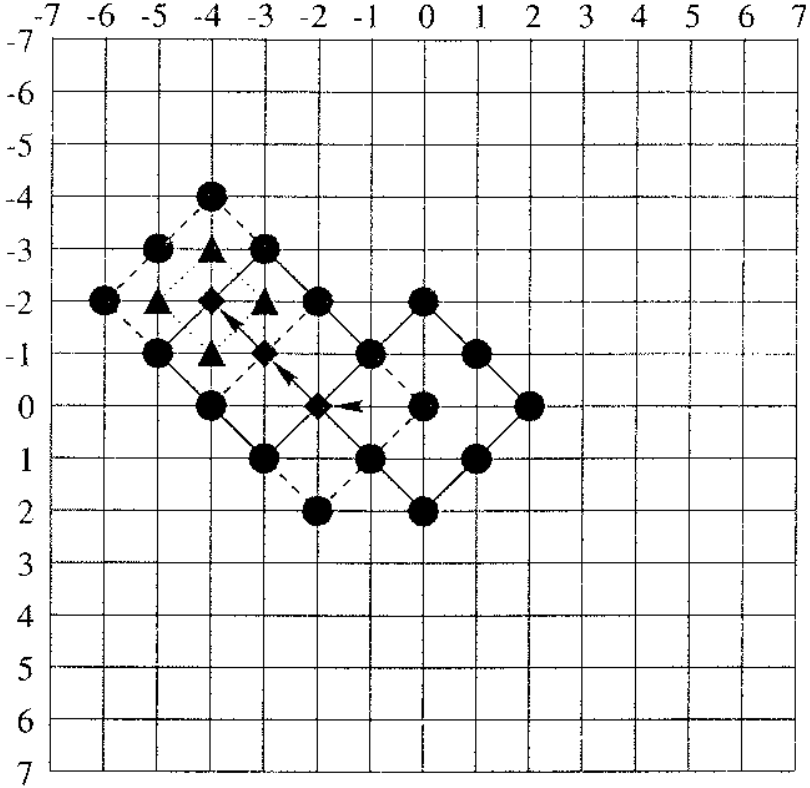
\includegraphics[keepaspectratio,width=.45\linewidth]{images/ds-exe.png}
        \caption{Example of a full execution cycle of diamond search}
    \end{figure}    
\end{frame}

\begin{frame}{DS results}
	\begin{figure}[H]
		\begin{minipage}[b]{0.45\textwidth}
            \centering
            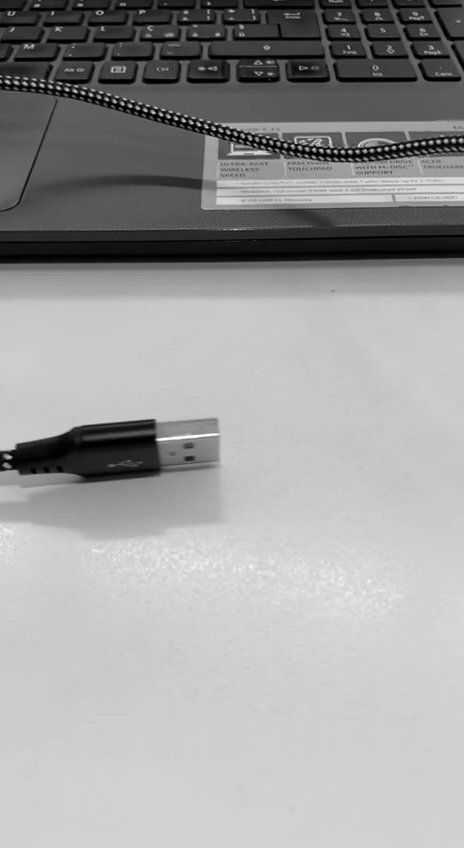
\includegraphics[keepaspectratio, width=.55\linewidth]{images/bbme-im.png}
            \label{fig:bbme-3-im}
            \subcaption{Target frame}
		\end{minipage}%
		\begin{minipage}[b]{0.45\textwidth}
            \centering
            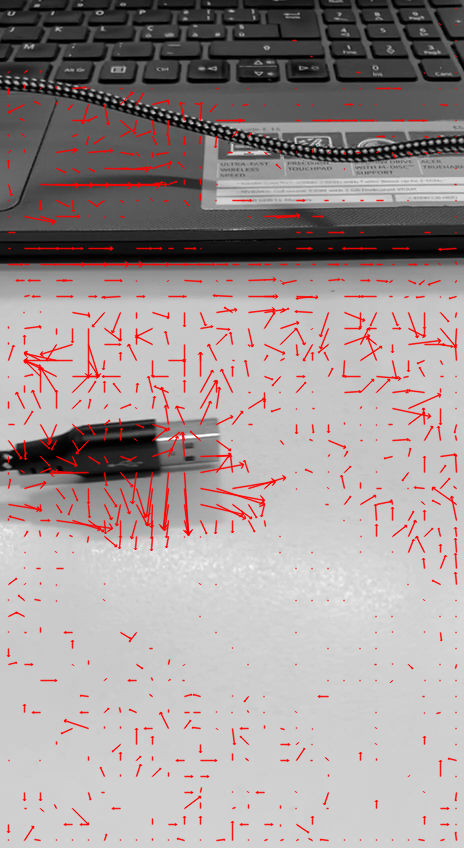
\includegraphics[keepaspectratio, width=.55\linewidth]{images/bbme-3-res.png}
            \label{fig:bbme-3-res}
            \subcaption{Needle diagram}
		\end{minipage}
        \label{fig:bbme-3}
        \caption{Motion field result of our DS implementation}
	\end{figure}
\end{frame}

\subsection{Global motion estimation}
\begin{frame}{Affine model prediction error}
    The affine model computes the displacement of a given pixel wrt parameters \(a\) as
    \begin{equation}
    \label{eq:displacement-matrix-formulation}
    d(p, a) = A(p)\;a
\end{equation}
    where \(A[p]\) is an intermediate matrix
    \begin{equation*}
    \label{eq:affine-model-parameter-matrix}
    A(p) = \begin{bmatrix}
        1 & x & y & 0 & 0 & 0 \\
        0 & 0 & 0 & 1 & x & y
    \end{bmatrix}
\end{equation*}
    \begin{block}{Fitting error}
        The fitting error computation gets rewritten as
        \begin{equation}
    \label{eq:pnorm-error}
    E = \sum_p{\left| d(p, a) - d(p) \right|^P}
\end{equation}
    \end{block}
\end{frame}

\begin{frame}{Affine model parameter estimation}
    We are interested in the parameters that minimize the fitting error \(\to \nabla_a E = 0\)
    \begin{block}{Parameter update}
        Assuming \(p = 2\), we get
        \begin{equation}
    \label{eq:optimal-parameter-affine}
    a = \left (\sum_p A[p]^T A[p] \right )^{-1} \left (\sum_p A[p]^T d(x) \right)
\end{equation}

    \end{block}
    \begin{exampleblock}{Refinement}
        \begin{itemize}
            \item each point \(p\) can be weighted
            \item parameter vector \(a\) can be split: \(a_x = [a_1,a_2,a_3]\) and \(a_y = [b_1,b_2,b_3]\)
            \begin{itemize}
                \item reduce the overall complexity
            \end{itemize}
        \end{itemize}
        \begin{equation}
    \footnotesize
    \label{eq:optimal-parameter-affine-weighted-halved}
    a_x = \left (\sum_p w(p) A_x[p]^T A_x[p] \right )^{-1} \left (\sum_p w(p) A_x[p]^T d_x(x) \right)
\end{equation}
    \end{exampleblock}
\end{frame}

\begin{frame}{Pseudocode}
    \begin{algorithm}[H]
    \DontPrintSemicolon
    
    \SetKwData{params}{\(a\)}
    \SetKwData{out}{outliers}
    \SetKwData{prevp}{prev\_pyrs}
    \SetKwData{curp}{cur\_pyrs}
    \SetKwData{prevf}{prev\_frame}
    \SetKwData{curf}{cur\_frame}
    \SetKwData{gt}{ground\_truth\_mfield}
    \SetKwData{est}{estimated\_mfield}
    
    \SetKwFunction{Pyr}{get\_pyr}
    \SetKwFunction{FirstEst}{first\_estimation}
    \SetKwFunction{Next}{next}
    \SetKwFunction{BM}{BBME}
    \SetKwFunction{Aff}{affine}
    \SetKwFunction{DetOut}{detect\_outliers}
    \SetKwFunction{Min}{minimize\_error}
    
    \KwIn{\textit{previous\_frame}, \textit{current\_frame}}
    \KwOut{\params \quad \texttt{//\(\;\)parameter vector}}
    \;        
    \prevp = \Pyr{previous\_frame}\;
    \curp = \Pyr{current\_frame}\;
    \params = \FirstEst{\prevp.\Next{}, \curp.\Next{}}\;
    \ForEach{\(l\) in levels}{
        \prevf = \prevp.\Next{}\;
        \curf = \curp.\Next{}\;
        \gt = \BM{\prevf, \curf}\;
        \est = \Aff{\params}\;
        \out = \DetOut{\gt, \est}\;
        \params = \Min{\prevf, \curf, \out}\;
        }
        
        \Return \params\;
        
        \caption{High-level pseudocode of our solution.}
        \label{alg:gme}
    \end{algorithm}


% prev_pyr = get_pyr(previous_frame)
% curr_pyr = get_pyr(current_frame)
% a = first_estimation(prev_pyr.pop(), curr_pyr.pop())
% for level in ([1,2]):
% 	curr = curr_pyr.pop()
% 	prev = prev_pyr.pop()
% 	ground_truth_mfield = BMME_motion_estimation(prev, curr)
% 	estimated_mfield = affine(a)
% 	outliers = detect_outliers(ground_truth_mfield, estimated_mfield)
% 	a = minimize_error(prev, curr, outliers)# update parameters
% return a 
\end{frame}

\section{Results}
\subsection{Qualitative: motion compensation}
\begin{frame}{Motion compensation}
    \begin{figure}[htbp]
        \begin{subfigure}[b]{0.3\textwidth}
            \centering
            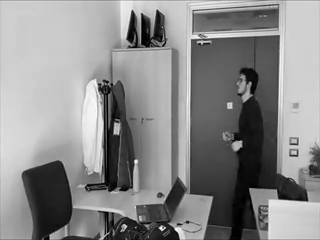
\includegraphics[width=.9\textwidth]{images/pan240-prev-frame.png}
            \caption{Previous frame}
            \label{fig:pan240-prev-frame}
        \end{subfigure}
        \hfill
        \begin{subfigure}[b]{0.3\textwidth}
            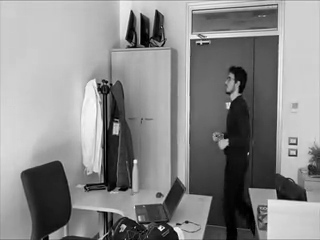
\includegraphics[width=.9\textwidth]{images/pan240-curr-frame.png}
            \caption{Next frame}
            \label{fig:pan240-curr-frame}
        \end{subfigure}
        \hfill
        \begin{subfigure}[b]{0.3\textwidth}
            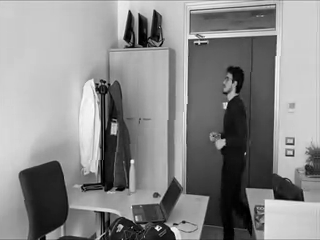
\includegraphics[width=.9\textwidth]{images/pan240-compensated.png}
            \caption{Compensated frame}
            \label{fig:pan240-compensated}
        \end{subfigure}
        
        \begin{subfigure}[b]{0.3\textwidth}
            \centering
            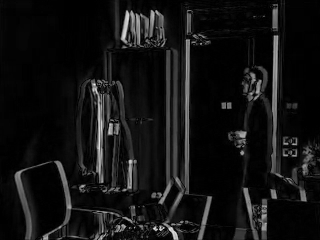
\includegraphics[width=.9\textwidth]{images/pan240-diff-curr-prev-1.png}
            \caption{Absolute difference between current and previous frame}
            \label{fig:pan240-diff-curr-prev}
        \end{subfigure}
        \hfill
        \begin{subfigure}[b]{0.3\textwidth}
            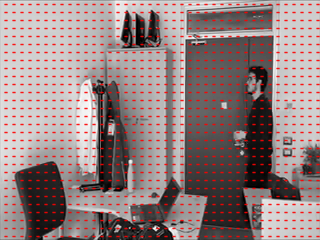
\includegraphics[width=.9\textwidth]{images/pan240-camera-motion-1.png}
            \caption{Global motion field estimated by our procedure}
            \label{fig:pan240-est-mf}
        \end{subfigure}
        \hfill
        \begin{subfigure}[b]{0.3\textwidth}
            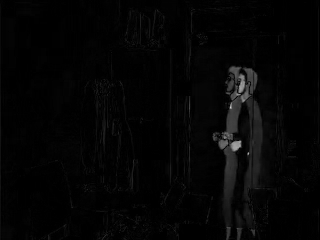
\includegraphics[width=.9\textwidth]{images/pan240-diff-curr-comp.png}
            \caption{Absolute difference between current and compensated frame}
            \label{fig:pan240-diff-curr-comp}
        \end{subfigure}
    
        \caption{Block size: 12, frame distance: 5}
    \end{figure}
\end{frame}

\begin{frame}{Motion compensation}
    \begin{figure}[htbp]
        \begin{subfigure}[b]{0.3\textwidth}
            \centering
            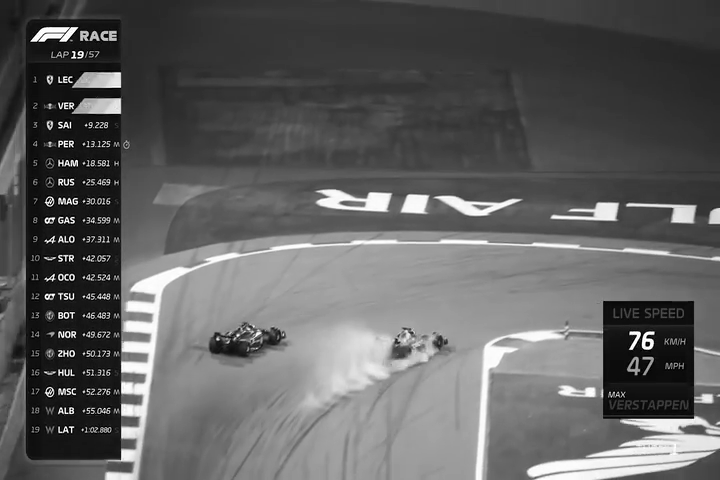
\includegraphics[width=.9\textwidth]{images/race-previous.png}
            \caption{Previous frame}
            \label{fig:race-prev-frame}
        \end{subfigure}
        \hfill
        \begin{subfigure}[b]{0.3\textwidth}
            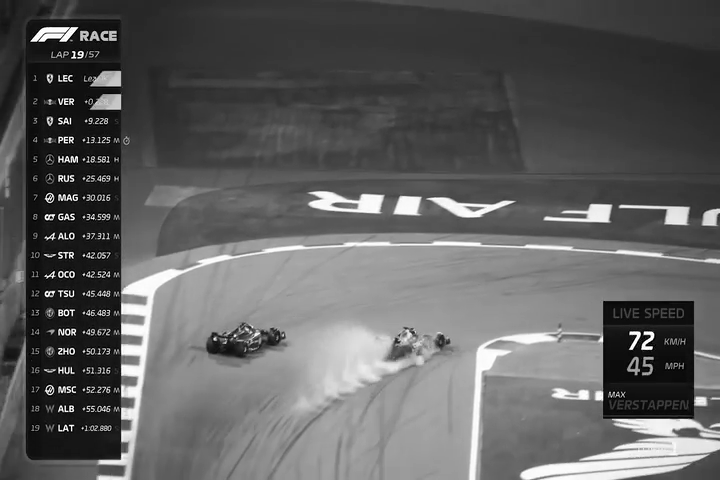
\includegraphics[width=.9\textwidth]{images/race-current.png}
            \caption{Next frame}
            \label{fig:race-curr-frame}
        \end{subfigure}
        \hfill
        \begin{subfigure}[b]{0.3\textwidth}
            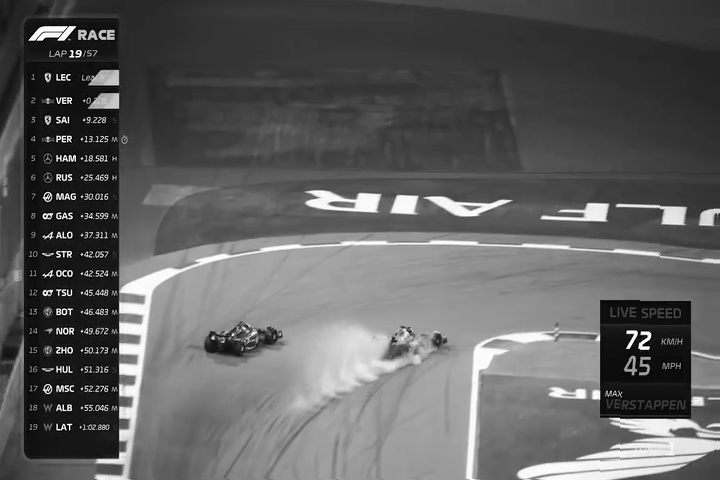
\includegraphics[width=.9\textwidth]{images/race-compensated.png}
            \caption{Compensated frame}
            \label{fig:race-compensated}
        \end{subfigure}
        
        \begin{subfigure}[b]{0.3\textwidth}
            \centering
            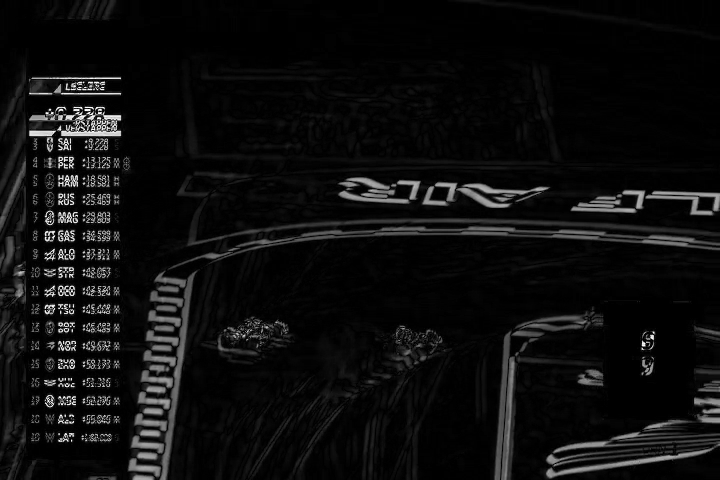
\includegraphics[width=.9\textwidth]{images/race-curr_prev_diff.png}
            \caption{Absolute difference between current and previous frame}
            \label{fig:race-diff-curr-prev}
        \end{subfigure}
        \hfill
        \begin{subfigure}[b]{0.3\textwidth}
            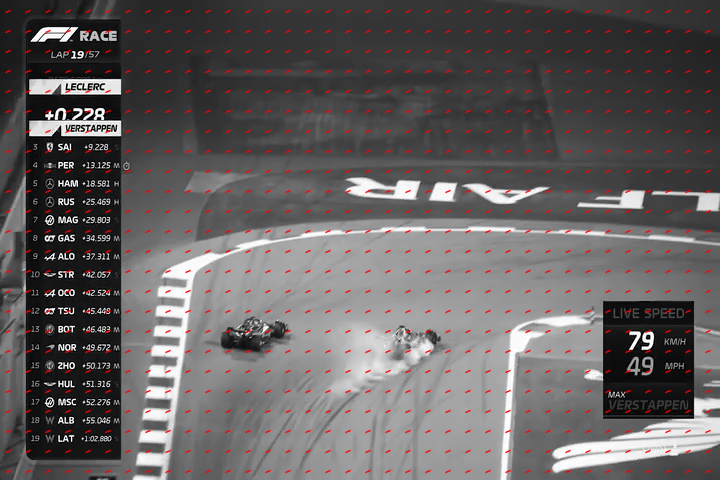
\includegraphics[width=.9\textwidth]{images/race-model_motion_field.png}
            \caption{Global motion field estimated by our procedure}
            \label{fig:race-est-mf}
        \end{subfigure}
        \hfill
        \begin{subfigure}[b]{0.3\textwidth}
            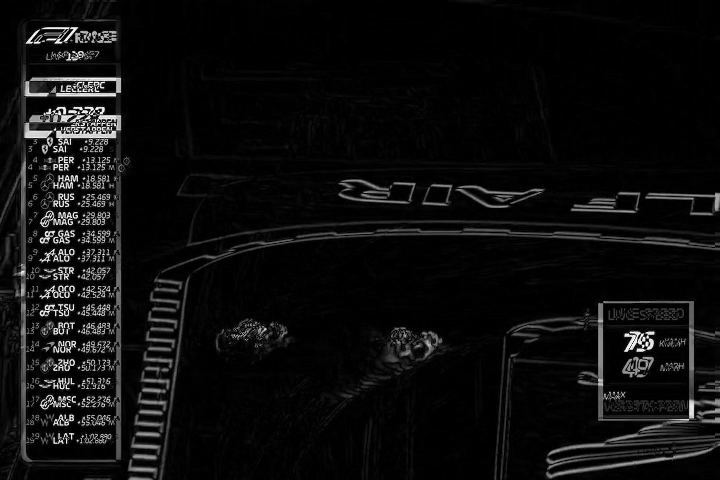
\includegraphics[width=.9\textwidth]{images/race-curr_comp_diff.png}
            \caption{Absolute difference between current and compensated frame}
            \label{fig:race-diff-curr-comp}
        \end{subfigure}
    
        \caption{Block size: 24, frame distance: 1}
    \end{figure}
\end{frame}

\begin{frame}{Motion compensation}
    \begin{figure}[htbp]
        \begin{subfigure}[b]{0.3\textwidth}
            \centering
            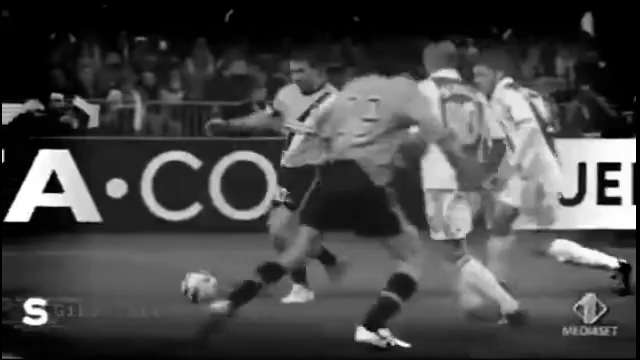
\includegraphics[width=\textwidth]{images/dp-previous.png}
            \caption{Previous frame}
            \label{fig:dp-prev-frame}
        \end{subfigure}
        \hfill
        \begin{subfigure}[b]{0.3\textwidth}
            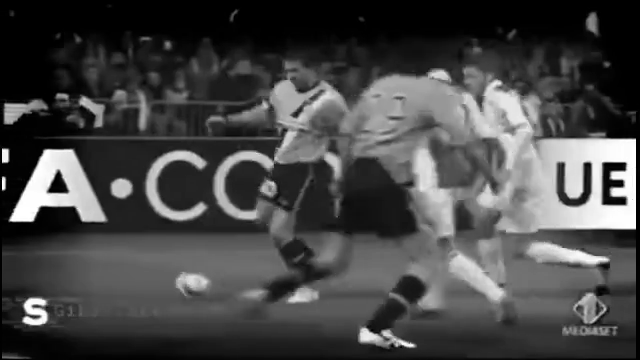
\includegraphics[width=\textwidth]{images/dp-current.png}
            \caption{Next frame}
            \label{fig:dp-curr-frame}
        \end{subfigure}
        \hfill
        \begin{subfigure}[b]{0.3\textwidth}
            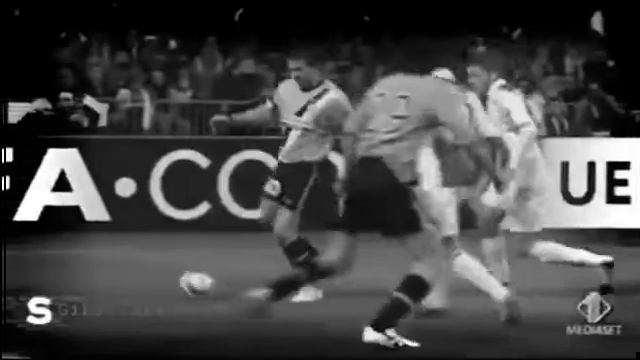
\includegraphics[width=\textwidth]{images/dp-compensated.png}
            \caption{Compensated frame}
            \label{fig:dp-compensated}
        \end{subfigure}
        
        \begin{subfigure}[b]{0.3\textwidth}
            \centering
            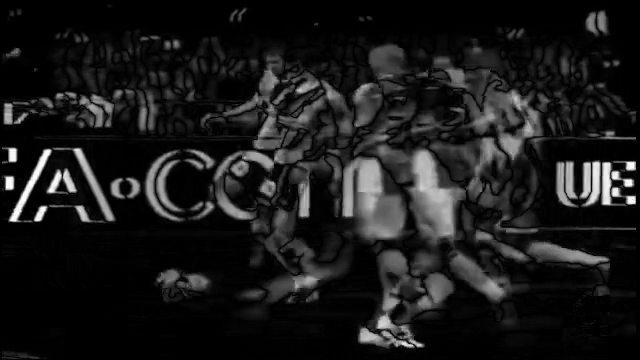
\includegraphics[width=\textwidth]{images/dp-curr_prev_diff.png}
            \caption{Absolute difference between current and previous frame}
            \label{fig:dp-diff-curr-prev}
        \end{subfigure}
        \hfill
        \begin{subfigure}[b]{0.3\textwidth}
            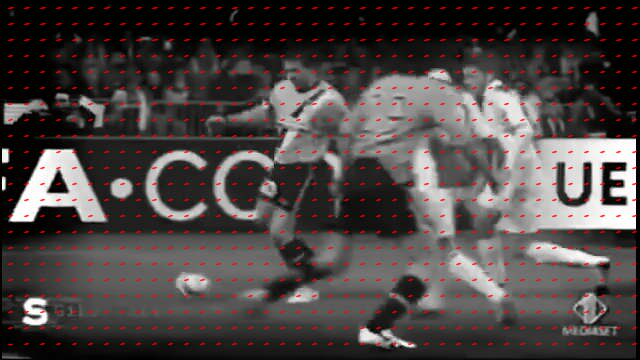
\includegraphics[width=\textwidth]{images/dp-model_motion_field.png}
            \caption{Global motion field estimated by our procedure}
            \label{fig:dp-est-mf}
        \end{subfigure}
        \hfill
        \begin{subfigure}[b]{0.3\textwidth}
            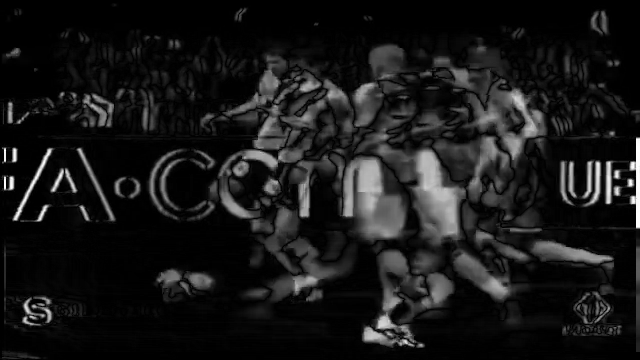
\includegraphics[width=\textwidth]{images/dp-curr_comp_diff.png}
            \caption{Absolute difference between current and compensated frame}
            \label{fig:dp-diff-curr-comp}
        \end{subfigure}
    
        \caption{Block size: 16, frame distance: 3}
    \end{figure}
\end{frame}

\begin{frame}{Motion compensation}
    \begin{figure}[htbp]
        \begin{subfigure}[b]{0.3\textwidth}
            \centering
            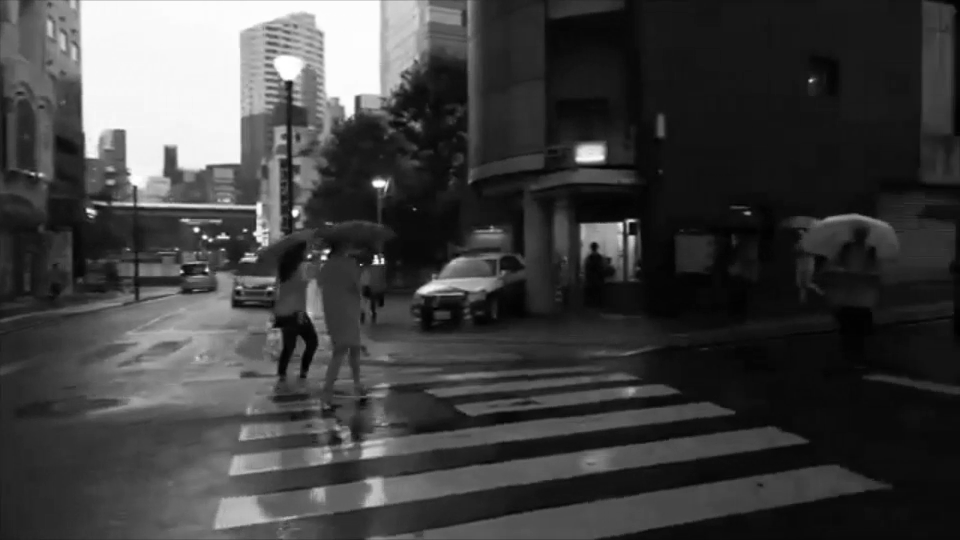
\includegraphics[width=\textwidth]{images/tokyo-previous.png}
            \caption{Previous frame}
            \label{fig:tokyo-prev-frame}
        \end{subfigure}
        \hfill
        \begin{subfigure}[b]{0.3\textwidth}
            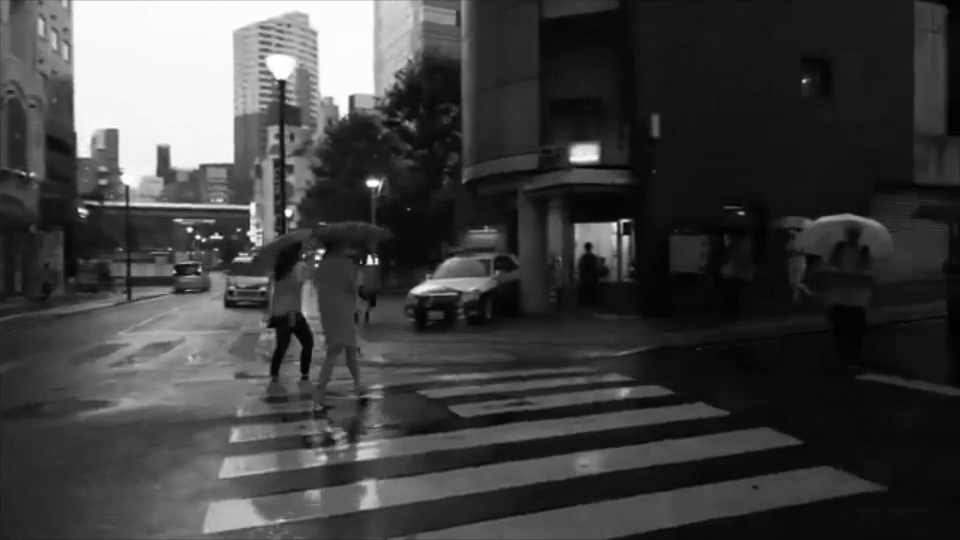
\includegraphics[width=\textwidth]{images/tokyo-current.png}
            \caption{Next frame}
            \label{fig:tokyo-curr-frame}
        \end{subfigure}
        \hfill
        \begin{subfigure}[b]{0.3\textwidth}
            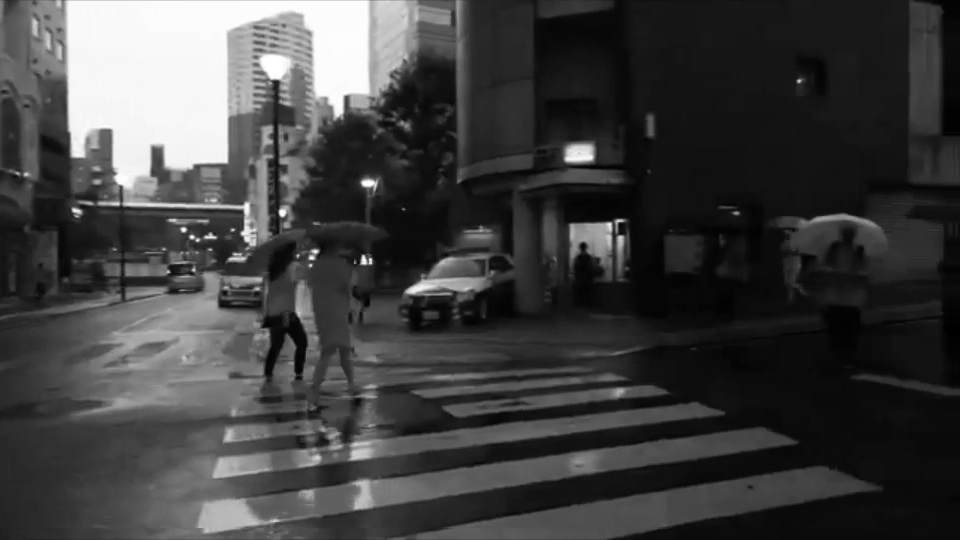
\includegraphics[width=\textwidth]{images/tokyo-compensated.png}
            \caption{Compensated frame}
            \label{fig:tokyo-compensated}
        \end{subfigure}
        
        \begin{subfigure}[b]{0.3\textwidth}
            \centering
            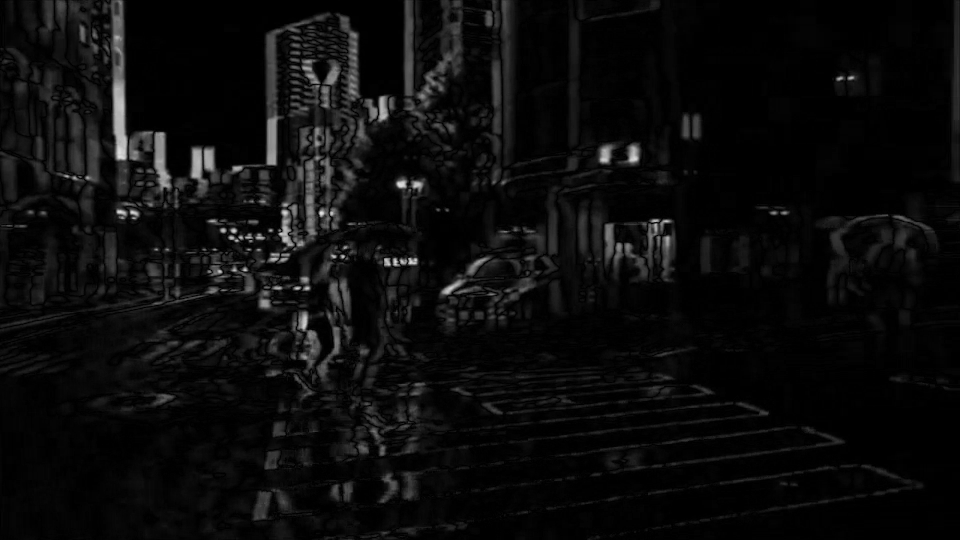
\includegraphics[width=\textwidth]{images/tokyo-curr_prev_diff.png}
            \caption{Absolute difference between current and previous frame}
            \label{fig:tokyo-diff-curr-prev}
        \end{subfigure}
        \hfill
        \begin{subfigure}[b]{0.3\textwidth}
            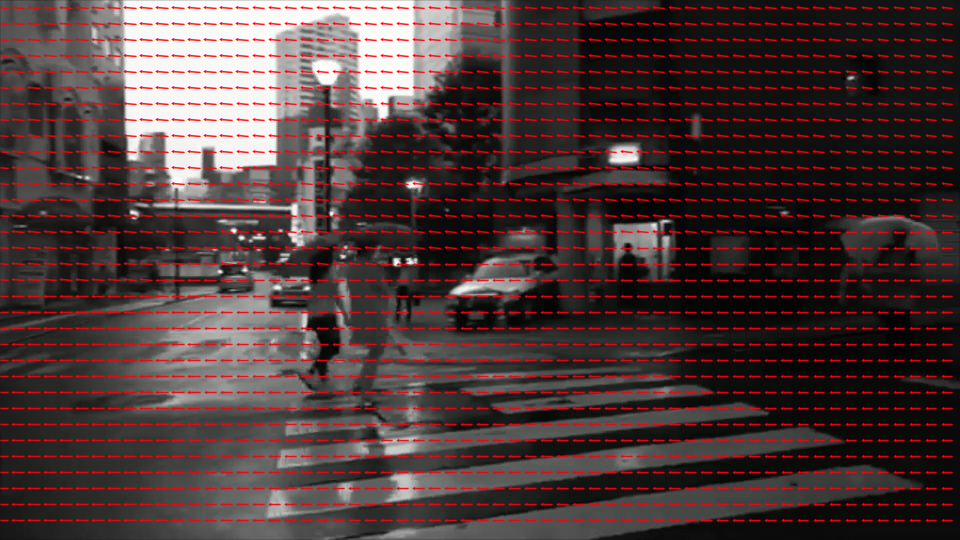
\includegraphics[width=\textwidth]{images/tokyo-model_motion_field.png}
            \caption{Global motion field estimated by our procedure}
            \label{fig:tokyo-est-mf}
        \end{subfigure}
        \hfill
        \begin{subfigure}[b]{0.3\textwidth}
            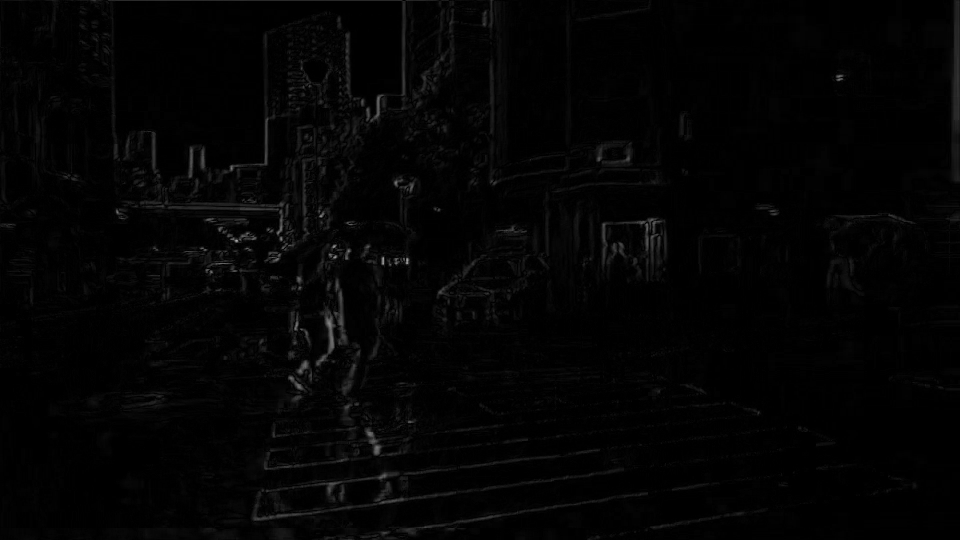
\includegraphics[width=\textwidth]{images/tokyo-curr_comp_diff.png}
            \caption{Absolute difference between current and compensated frame}
            \label{fig:tokyo-diff-curr-comp}
        \end{subfigure}
    
        \caption{Block size: 16, frame distance: 1}
    \end{figure}
\end{frame}

\begin{frame}{Motion compensation}
    \begin{figure}[htbp]
        \begin{subfigure}[b]{0.3\textwidth}
            \centering
            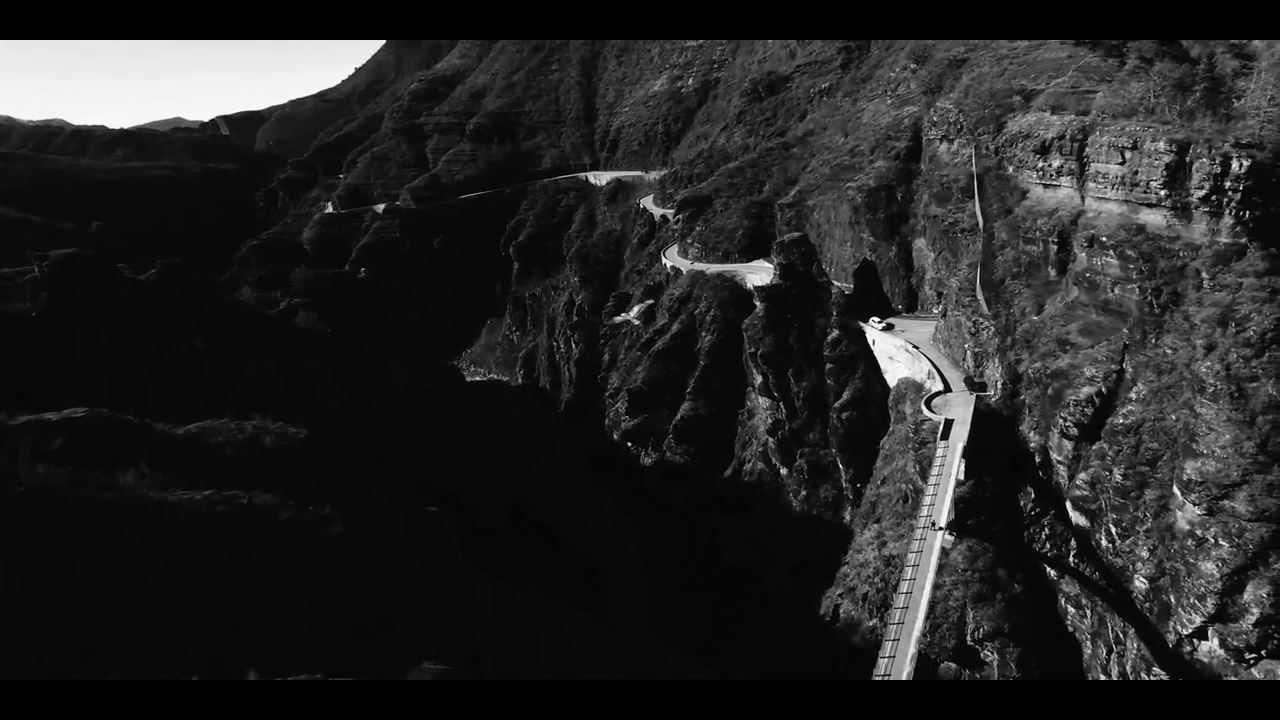
\includegraphics[width=\textwidth]{images/bird-previous.png}
            \caption{Previous frame}
            \label{fig:bird-prev-frame}
        \end{subfigure}
        \hfill
        \begin{subfigure}[b]{0.3\textwidth}
            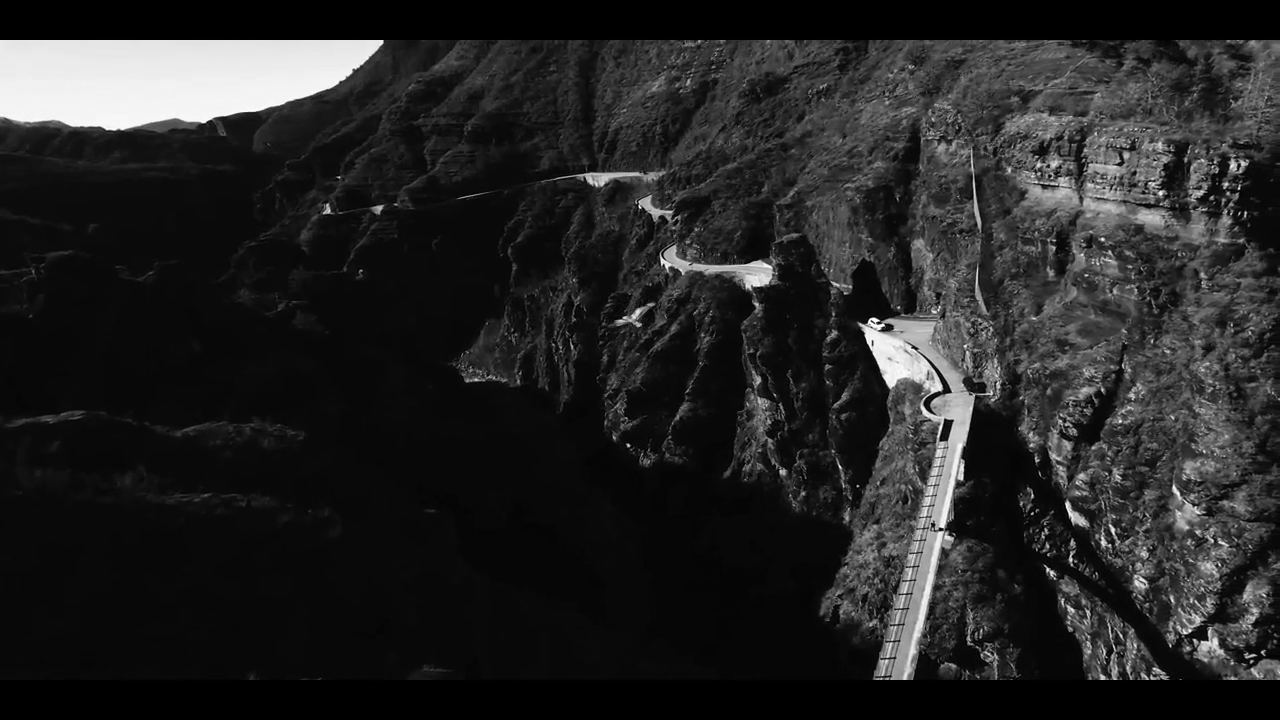
\includegraphics[width=\textwidth]{images/bird-current.png}
            \caption{Next frame}
            \label{fig:bird-curr-frame}
        \end{subfigure}
        \hfill
        \begin{subfigure}[b]{0.3\textwidth}
            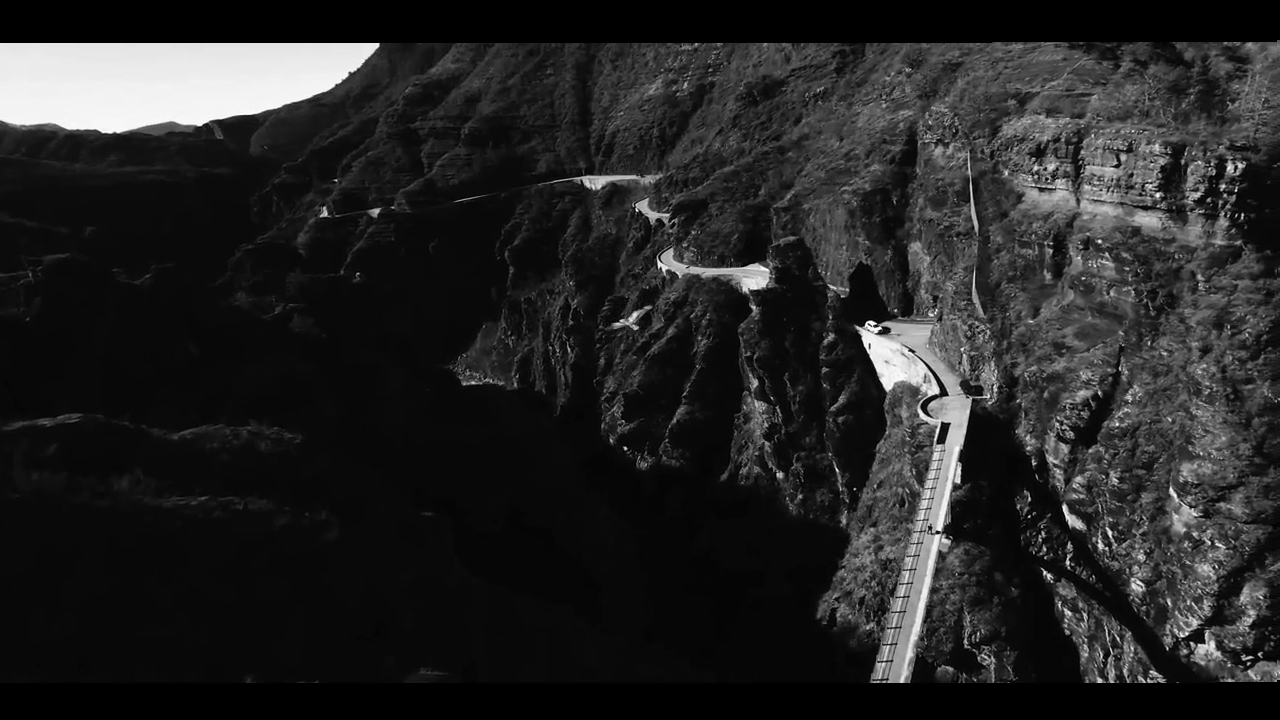
\includegraphics[width=\textwidth]{images/bird-compensated.png}
            \caption{Compensated frame}
            \label{fig:bird-compensated}
        \end{subfigure}
        
        \begin{subfigure}[b]{0.3\textwidth}
            \centering
            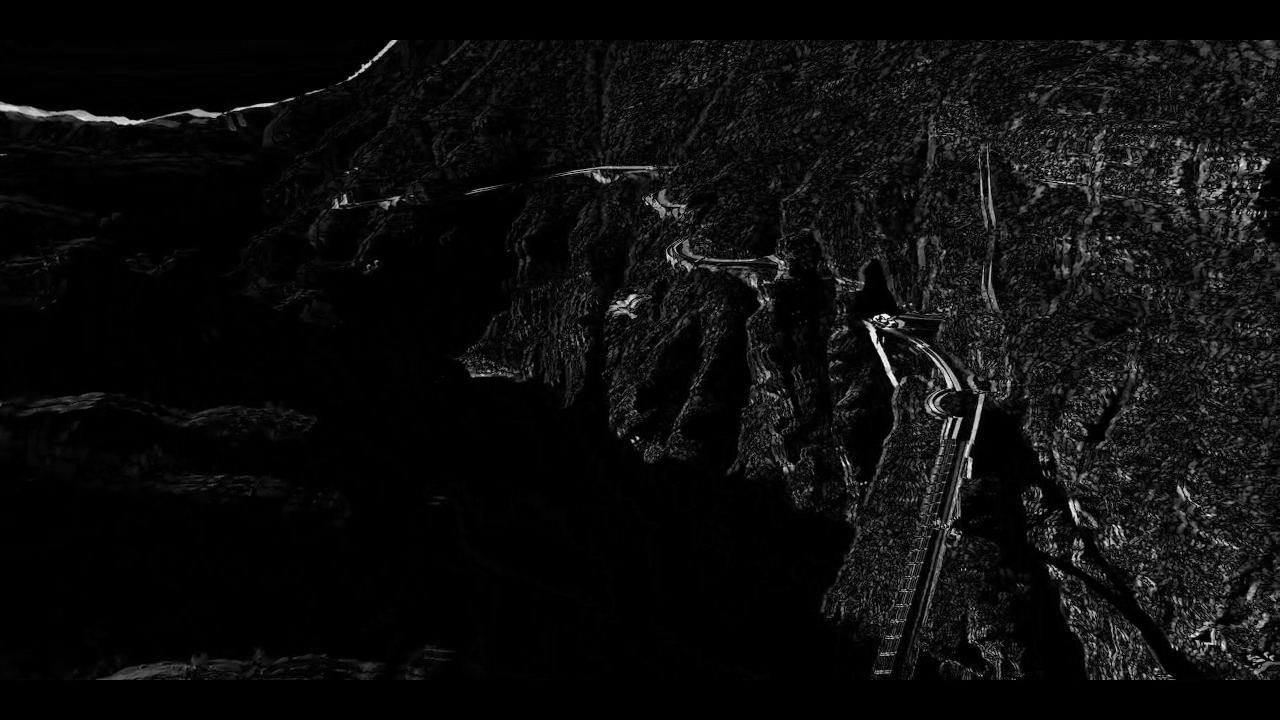
\includegraphics[width=\textwidth]{images/bird-curr_prev_diff.png}
            \caption{Absolute difference between current and previous frame}
            \label{fig:bird-diff-curr-prev}
        \end{subfigure}
        \hfill
        \begin{subfigure}[b]{0.3\textwidth}
            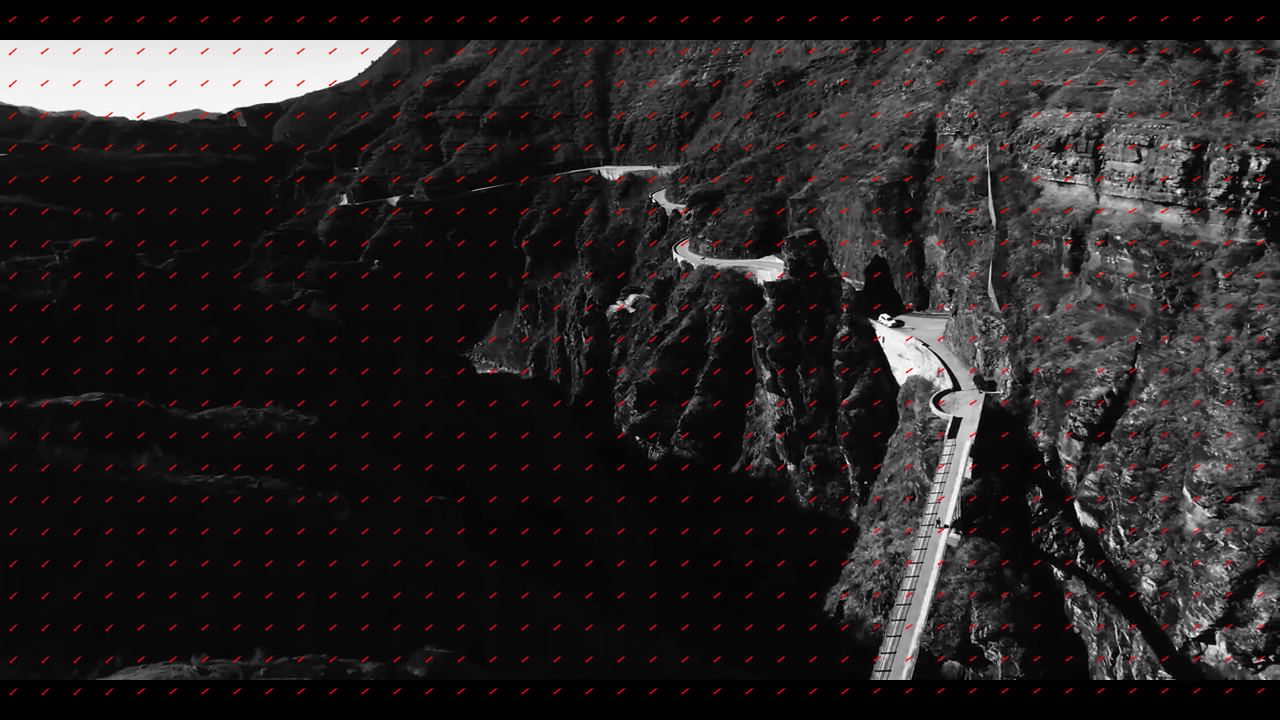
\includegraphics[width=\textwidth]{images/bird-model_motion_field.png}
            \caption{Global motion field estimated by our procedure}
            \label{fig:bird-est-mf}
        \end{subfigure}
        \hfill
        \begin{subfigure}[b]{0.3\textwidth}
            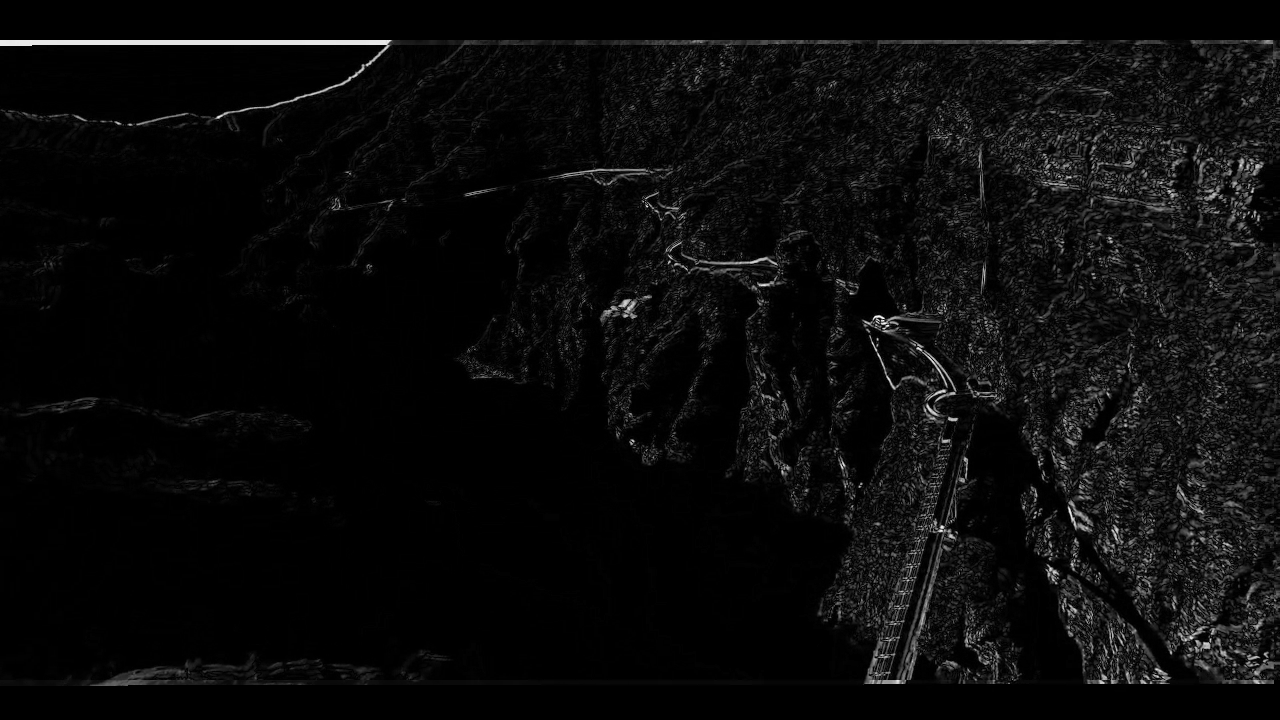
\includegraphics[width=\textwidth]{images/bird-curr_comp_diff.png}
            \caption{Absolute difference between current and compensated frame}
            \label{fig:bird-diff-curr-comp}
        \end{subfigure}
    
        \caption{Block size: 32, frame distance: 1}
    \end{figure}
\end{frame}

\subsection{Quantitative: PSNR}
\begin{frame}{PSNR results}
    \begin{table}
        \label{tab:psnr}
        \begin{tabular}{ll|rrrr}
    \toprule
    Video & Properties & Average & Variance & Maximum & Minimum \\
    \midrule
    {\small\texttt{pan240.mp4}} & {\small Fast motion} & \(22.724\)  & \(5.125\)  & \(27.802\) & \(17.981\)  \\

    {\small\texttt{coastguard\_qcif.mp4}} & 
        \begin{tabular}{@{}c@{}}{\small Two objects moving,}\\{\small background moving}\end{tabular}
    & \(22.733\)  & \(2.194\)  & \(26.875\) & \(15.158\)  \\
    
    {\small\texttt{foreman.mp4}} & 
        \begin{tabular}{@{}c@{}}{\small Big object moving,}\\{\small still background}\end{tabular}
        & \(19.677\)  & \(18.443\)  & \(30.436\) & \(11.746\)  \\
        
    {\small\texttt{numeri\_del\_piero.mp4}} & 
        \begin{tabular}{@{}c@{}}{\small Medium object moving,}\\{\small moving background}\end{tabular}
    & \(19.072\)  & \(13.642\)  & \(47.722\) & \(16.323\)  \\
    

    \bottomrule
\end{tabular}
        \caption{PSNR result on a some example video sequences}
    \end{table}    
\end{frame}


\section{Conclusions}
\begin{frame}
    \begin{block}{Summary}
        In this work, we have presented:
        \begin{itemize}
            \item a broad introduction to the problem of global motion estimation
            \item an in-depth explanation of the theoretical foundations of our solution
            \item the framework we developed from the aforementioed literature
            \begin{itemize}
                \item the BBME algorithms chosen
                \item the computation of the parameter for the affine model
                \item the removal of outliers
                \item the implementation of the multiscale approach
            \end{itemize}
            \item an analysis of the results of our solution
            \begin{itemize}
                \item qualitative results, using motion compensation
                \item quantitative results, comparing PSNR values
            \end{itemize} 
        \end{itemize}        
    \end{block}
\end{frame}

\end{document}